%% abtex2-modelo-projeto-pesquisa.tex, v<VERSION> laurocesar
%% Copyright 2012-2015 by abnTeX2 group at http://www.abntex.net.br/ 
%% 
%% This work may be distributed and/or modified under the
%% conditions of the LaTeX Project Public License, either version 1.3
%% of this license or (at your option) any later version.
%% The latest version of this license is in
%% http://www.latex-project.org/lppl.txt
%% and version 1.3 or later is part of all distributions of LaTeX
%% version 2005/12/01 or later.
%% 
%% This work has the LPPL maintenance status `maintained'.
%% 
%% The Current Maintainer of this work is the abnTeX2 team, led
%% by Lauro César Araujo. Further information are available on 
%% http://www.abntex.net.br/
%% 
%% This work consists of the files abntex2-modelo-projeto-pesquisa.tex
%% and abntex2-modelo-references.bib
%% 

% ------------------------------------------------------------------------
% ------------------------------------------------------------------------
% abnTeX2: Modelo de Projeto de pesquisa em conformidade com 
% ABNT NBR 15287:2011 Informação e documentação - Projeto de pesquisa -
% Apresentação 
% ------------------------------------------------------------------------ 
% ------------------------------------------------------------------------

\documentclass[
% -- opções da classe memoir --
12pt,				% tamanho da fonte
openright,			% capítulos começam em pág ímpar (insere página vazia caso preciso)
oneside,			% para impressão em recto e verso. Oposto a oneside
a4paper,			% tamanho do papel. 
% -- opções da classe abntex2 --
% chapter=TITLE,		% títulos de capítulos convertidos em letras maiúsculas
% section=TITLE,		% títulos de seções convertidos em letras maiúsculas
% subsection=TITLE,	% títulos de subseções convertidos em letras maiúsculas
% subsubsection=TITLE,% títulos de subsubseções convertidos em letras maiúsculas
% -- opções do pacote babel --
english,			% idioma adicional para hifenização
brazil,				% o último idioma é o principal do documento
]{abntex2}


% ---
% PACOTES
% ---

% ---
% Pacotes fundamentais 
% ---
\usepackage{lmodern}			% Usa a fonte Latin Modern
\usepackage[T1]{fontenc}		% Selecao de codigos de fonte.
\usepackage[utf8]{inputenc}		% Codificacao do documento (conversão automática dos acentos)
\usepackage{indentfirst}		% Indenta o primeiro parágrafo de cada seção.
\usepackage{color}				% Controle das cores
\usepackage{graphicx}			% Inclusão de gráficos
\usepackage{microtype} 			% para melhorias de justificação
\usepackage{amsmath,amssymb,amstext}
\usepackage{setspace}

% ---
% Pacotes e definições adcionais, para adequações especificas
\usepackage{tikz}				
\usepackage{pdflscape}			% para ambiente landscape
\usepackage{pgfgantt}			% cronograma estilo gráfico de gantt
\usetikzlibrary{backgrounds}
\definecolor{done}{RGB}{120, 180, 120}
\definecolor{do}{RGB}{180, 120, 120}

% ---

% ---
% Pacotes adicionais, usados apenas no âmbito do Modelo Canônico do abnteX2
% ---
\usepackage{lipsum}				% para geração de dummy text
% ---

% ---
% Pacotes de citações
% ---
\usepackage[brazilian,hyperpageref]{backref}% Paginas com as citações
\usepackage[alf]{abntex2cite}				% Citações padrão ABNT

% --- 
% CONFIGURAÇÕES DE PACOTES
% --- 

% ---
% Configurações do pacote backref
% Usado sem a opção hyperpageref de backref
\renewcommand{\backrefpagesname}{Citado na(s) página(s):~}
% Texto padrão antes do número das páginas
\renewcommand{\backref}{}
% Define os textos da citação
\renewcommand*{\backrefalt}[4]{
  \ifcase #1 %
  Nenhuma citação no texto.%
  \or
  Citado na página #2.%
  \else
  Citado #1 vezes nas páginas #2.%
  \fi}%
% ---

% ---
% Informações de dados para CAPA e FOLHA DE ROSTO
% ---
\titulo{Extensões e Aplicações Modelo de Regressão
  Conway-Maxwell-Poisson para Modelagem de Dados de Contagem}
\vspace{2cm}
\autor{Eduardo Elias Ribeiro Junior}
\local{Curitiba}
\data{2015}
\instituicao{Universidade Federal do Paraná
  \par
  Setor de Ciências Exatas
  \par
  Departamento de Estatística
}
\orientador[Orientador:]{Prof. Dr. Walmes Marques Zeviani}
\tipotrabalho{Projeto de Pesquisa}
% O preambulo deve conter o tipo do trabalho, o objetivo, 
% o nome da instituição e a área de concentração 
\preambulo{Projeto de Pesquisa apresentado à disciplina Laboratório A 
  do Curso de Graduação em Estatística da Universidade Federal do Paraná, 
  como requisito para elaboração do Trabalho de Conclusão de Curso}
% ---

% ---
% Configurações de aparência do PDF final

% alterando o aspecto da cor azul
\definecolor{blue}{RGB}{41,5,195}

% informações do PDF
\makeatletter
\hypersetup{
  % pagebackref=true,
  pdftitle={\@title}, 
  pdfauthor={\@author},
  pdfsubject={\imprimirpreambulo},
  pdfcreator={LaTeX with abnTeX2},
  pdfkeywords={abnt}{latex}{abntex}{abntex2}{projeto de pesquisa}, 
  colorlinks=true,	% false: boxed links; true: colored links
  linkcolor=blue,     % color of internal links
  citecolor=blue, % color of links to bibliography
  filecolor=magenta, % color of file links
  urlcolor=blue,
  bookmarksdepth=4
}
\addto\captionsbrazil{
  \renewcommand{\bibname}{REFER\^ENCIAS}
}
\makeatother
% --- 

% --- 
% Espaçamentos entre linhas e parágrafos 
% --- 

% O tamanho do parágrafo é dado por:
\setlength{\parindent}{1.3cm}

% Controle do espaçamento entre um parágrafo e outro:
\setlength{\parskip}{0.2cm}  % tente também \onelineskip

% ---
% compila o indice
% ---
\makeindex
% ---

% ----
% Início do documento
% ----
\begin{document}

% Seleciona o idioma do documento (conforme pacotes do babel)
% \selectlanguage{english}
\selectlanguage{brazil}

% Retira espaço extra obsoleto entre as frases.
% \frenchspacing 

% ----------------------------------------------------------
% ELEMENTOS PRÉ-TEXTUAIS
% ----------------------------------------------------------
% \pretextual

% ---
% Capa
% ---
\tikz[remember picture,overlay] \node[opacity=0.9,inner sep=0pt] at 
(current page.center){
  \includegraphics[width=\paperwidth,
  height=\paperheight]{figures/ufpr_bg}};

\begin{center}
  {\Large \textsf{Universidade Federal do Paraná}} \\
\end{center}
\imprimircapa

% ---

% ---
% Folha de rosto
% ---
\imprimirfolhaderosto
% ---

% ---
% inserir o sumario
% ---
\pdfbookmark[0]{\contentsname}{toc}
\tableofcontents*
\cleardoublepage
% ---


% ----------------------------------------------------------
% ELEMENTOS TEXTUAIS
% ----------------------------------------------------------
\textual

% ----------------------------------------------------------
% Introdução
% ----------------------------------------------------------
\chapter{Introdução}
\label{cha:introducao}

Modelos estatísticos de regressão são fundamentalmente os principais
métodos suporte para a prática de Estatística aplicada. Diversas áreas
do conhecimento são familiares a estes modelos, pois eles objetivam
descrever a relação entre uma variável dependente, de interesse, com
variáveis independentes, a fim de compreender este relacionamento e
realizar predições através do modelo estabelecido, principal interesse
de pesquisas aplicadas. Um modelo estatístico, na sua forma univariada
consiste no estabelecimento de um equação matemática que relaciona uma
variável de interesse $Y$ com variáveis preditoras $X_i$, considerando
uma distribuição de probabilidades para $Y$ condicionalmente à $X$ e 
de média associada a um preditor linear dos efeitos das variáveis
independentes.

Podemos destacar o modelo linear normal, com distribuição Normal
associada à $[Y \mid X]$ e preditor linear da forma $X\beta$, como o
modelo predominante dentre as análises estatísticas aplicadas. Até a
década de 70, para situações em que a variável resposta $Y$ não se
apresentava de forma contínua com domínio nos reais ou ainda não se
verificava os pressupostos do modelo, a alternativa mais utilizada era
encontrar alguma forma de transformação da variável resposta para
atingir a normalidade \cite{Paula2013}. Porém, com a introdução dos
da teoria do modelos lineares generalizados (MLG) por
\citeauthoronline{Nelder1972} (\citeyear{Nelder1972}) e com o avanço
computacional, a análise de dados não normais passou a ser
corriqueiramente via MLG's. Esta nova classe de modelos flexibiliza a 
distribuição condicional associada, permitindo outras distribuições
pertencentes à família exponencial de distribuições o que contempla as
distribuições Normal, Poisson, Binomial, Gama entre outras bem
conhecidas na literatura. 

Com isso a modelagem de dados passou a ser mais
fiel a natureza dos dados em observação. Neste contexto, a análise de
variáveis aleatórias de contagem, que representam o número de
ocorrências de um evento de interesse em um intervalo de tempo ou espaço
específico, foi enriquecida expressivamente. Pois via o modelo
linear normal as estimativas contêm erros padrão inconsistentes e podem
produzir predições negativas para o número de eventos
\cite{King1989}. 

Para análise estatística destas variáveis temos o modelo probabilístico
de Poisson, já consolidado na literatura, sendo amplamente
utilizado. Este modelo possui apenas um parâmetro, denotado por
$\lambda$ que atua na média e na variância a partir de uma relação
identidade ($\lambda = E[Y] = V[Y]$). Essa propriedade, chamada de
equidispersão, é uma particularidade do modelo Poisson que pode não ser
adequada a diversas situações. Quando aplicado sem verificação desta
suposição, o modelo Poisson acarreta em erros padrões inconsistentes.

Algumas abordagens para modelagem de dados de contagens com fuga de
equidispersão foram propostas na literatura. O caso de superdispersão,
quando a variância é maior que a média é o mais comum e tem uma gama de
métodos para análise mais extensa. A superdispersão pode ocorrer pela
ausência de covariáveis importantes, excesso de zeros, diferentes
amplitudes de domínio (\textit{offset}) não considerado, heterogeneidade
de unidades amostrais, excesso de zeros, entre
outros \cite{RibeiroJr2012}. Para estes casos a abordagem mais comum é a
adoção de modelos com efeitos aleatórios que capturam a variabilidade
extra. Um caso particular dos modelos Poisson de efeitos aleatórios,
muito adotado no campo aplicado da Estatística, ocorre quando
consideramos distribuição Gama para os efeitos aleatórios, nesta
situação temos expressão fechada para a função de probabilidade marginal
que assume a forma Binomial Negativa. Contudo outra manifestação de
fuga da suposição de equidispersão é a subdispersão, situação menos
comum na literatura. O processo
que reduz a variabilidade das contagens Poisson não é tão claro quanto o
que produz variabilidade extra e é muito particular do experimento em
estudo. São poucas as abordagens descritas na literatura  que
compreendem o tratamento de
subdispersão, uma vez que efeitos aleatórios só capturam avariabilidade
extra. Podemos citar os modelos de quase-verossimilhança como a 
abordagem mais utilizada, todavia não é possível recuperar a verdadeira
distribuição da variável resposta nesta abordagem pois aqui a
modelagem é baseada apenas nos dois primeiros momentos \cite{Paula2013}. 

Anteriormente à formalização dos MLG's, em um contexto de filas
\citeauthoronline{Conway1962} (\citeyear{Conway1962}) propuseram uma
distribuição de probabilidades que 
generaliza a distribuição Poisson com a adição de mais uma parâmetro,
denotado por $\nu$, contemplando agora os casos de sub e
superdispersão. Posteriormente esta distribuição foi nomeada como 
COM-Poisson (Conway-Maxwell-Poisson em homenagem à Richard W. Conway,
William L. Maxwell seus autores). A função distribuição de probabilidade
COM-Poisson assume a forma

\begin{equation} \label{eq:dcmp}
  P(Y = y) = \frac{\lambda^y}{(y!)^\nu} \frac{1}{Z(\lambda, \nu)}, \qquad
  y \in \mathbb{Z}_+
\end{equation}

\noindent
onde $Z(\lambda, \nu) = \sum_{j=0}^\infty \frac{\lambda^s}{(s!)^\nu}$,
$\lambda > 0$ e $\nu \geq 0$. A flexibilidade da COM-Poisson é
verificada pela razão de probabilidades consecutivas, que se caracteriza
não necessariamente linear em $y$ ($P(Y = y - 1) / P(Y = y) = y^\nu /
\lambda$) sendo governada pelo parâmetro extra $\nu$
\cite{Shmueli2005}. Uma característica bastante relevante é que esta
distribuição 
pertence à família exponencial e possui como casos particulares as
distribuições Poisson, Geométrica e Binomial. Portanto, empregando a
distribuição COM-Poisson na estrutura de um MLG obtemos um modelo de
regressão sem a imposição de equidispersão. 

A aplicação do modelo de regressão COM-Poisson não apresenta forma
analítica para estimação, portanto métodos numéricos são empregados
nesta tarefa. Ainda a constante normalizadora $Z(\lambda, \nu)$ em
\ref{eq:dcmp} se apresenta como uma série infinita que
computacionalmente deve ser truncada. Algumas aplicações do modelo
de regressão COM-Poisson são apresentadas em \citeonline{Shmueli2005} e
\citeonline{Sellers2010}.

Pela similaridade da função de distribuição COM-Poisson em \ref{eq:dcmp}
com a Poisson vários aspectos podem ser estendidos. Por exemplo, citamos
a inclusão de efeitos aleatórios para acomodar superdispersão, porém há
situações em que o delineamento do experimento sugere a correlação entre
observações de parcelas da amostra e independência entre parcela. São
efeitos não observáveis que agem no nível de observação e isso pode ser
incorporado no modelo de regressão COM-Poisson. Da mesma forma excesso
de zeros podem ser introduzidos a esta distribuição da mesma forma com o
que ocorre para o modelo Poisson, através de truncamento (modelos
Hurdle) ou inflação (modelos de mistura). Estas extensões citadas para o
modelo COM-Poisson não são bem consolidadas na literatura e são raras
suas aplicações. Uma constatação do fato é que não há implementações
destas extensões nos principais softwares estatísticos.

Na literatura brasileira a aplicação dos modelos COM-Poisson são
escassos. Foram encontrados apenas aplicações na área de Análise de
Sobrevivência mais especificamente em modelos com fração de
cura. Portanto a presente pesquisa visa colaborar com a literatura
estatística brasileira apresentando e explorando alternativas para
modelagem de dados de contagem e suas extensões para situações comuns em
estudos experimentais e observacionais.

% ----------------------------------------------------------
% Objetivos
% ----------------------------------------------------------
\chapter{Objetivos}
\label{cha:objetivos}

\section{Objetivos Gerais}
\label{sec:objetivosgerais}

Apresentar o modelo de regressão COM-Poisson, alternativa 
paramétrica não comumente utilizada pela comunidade de 
Estatística aplicada, trazendo discussões sobre aspectos 
inferenciais deste modelo. Estender as aplicações do modelo
COM-Poisson para situações específicas (efeitos aleatórios 
e excesso de zeros).

\section{Objetivos Específicos}
\label{sec:objetivosespecificos}

\begin{itemize}
\item Apresentar e discutir aspectos da distribuição COM-Poisson para
  modelos de regressão para dados de contagem;
  
\item Avaliar as propriedades de soluções numéricas para 1) cálculo da
  densidade de probabilidade do modelo e 2) para estimação de modelos de 
  regressão de efeito fixo;
  
\item Propor e implementar uma extensão do modelo de regressão
  COM-Poisson para acomodar efeitos aleatórios;
  
\item Propor e implementar uma extensão do modelo de regressão
  COM-Poisson para acomodar contagens com excesso de zeros.
  
\item Fazer a aplicação do modelo COM-Poisson e das extensões
  desenvolvidas à dados reais ou simulados. Fazer comparações com os
  modelos disponíveis para as situações estudadas: Poisson,
  Quase-Poisson, Binomial Negativo, Poisson de efeito aleatório.
\end{itemize}

% ----------------------------------------------------------
% Materiais e Métodos
% ----------------------------------------------------------
\chapter{Materiais e Métodos}
\label{cha:materiaisemetodos}

\section{Materiais}
\label{sec:materiais}

\subsection{Dados para análise}
\label{sec:dados}

Este projeto de pesquisa via o estudo e avaliação do modelo de regressão
COM-Poisson para modelagem de dados de contagem. Portanto pretende-se
analisar vários conjuntos de dados, preferencialmente os já analisados
na literatura via outras técnicas, para efeitos de comparação.

Inicialmente temos o conjunto \texttt{defoliation}, disponível no
\textit{software} R através do pacote \texttt{legTools}\footnote{Em
  desenvolvimento pelo Laboratório de Estatística e Geoinformação da
  UFPR \url{http://git.leg.ufpr.br/leg/legTools}}. Este conjunto de
dados contém 125 observações provenientes de um experimento em casa de
vegetação inteiramente casualizado com 5 repetições, cujo plantas de
algodão (\textit{Gossypium hirsutum}) foram submetidas à níveis de
desfolha artificial (5 níveis) combinados com o estágio fenológico da
planta na aplicação da desfolha (5 níveis), observou-se como variável
resposta o número de capulhos produzidos ao final do ciclo cultura. Este
conjunto de dados foi analisado considerando o modelo de contagem Gamma
por \citeonline{Zeviani2014}.

Ainda serão utilizados dados simulados para avaliação da acurácia dos
métodos de estimação e comparação de abordagens distintas em diferentes
cenários.

\subsection{Recursos Computacionais}
\label{sec:recursos}

Para análise e elaboração do trabalho será utilizado o
\textit{software R}, na versão 3.2 \cite{Rcore2015}. 
Atualmente há três bibliotecas desenvolvidas em R dedicadas
à distribuição COM-Poisson. São eles \texttt{COMPoissonReg}
\cite{COMPoissonReg}, este conjunto de funções foi 
desenvolvido com base nas análises apresentadas no artigo
\textit{A flexible regression model for count data} 
\cite{Sellers2010}; \texttt{compoisson} as funções desta 
biblioteca se dedicam apenas ao modelo probabilístico; e
\texttt{CompGLM} esta é mais recente biblioteca de funções 
com ênfase no modelo COM-Poisson, escrita em \texttt{C++}
permite a estimação de modelos de regressão além de funções 
probabilísticas.

Outros recursos e bibliotecas, principalmente para 
otimização de funções e elaboração de gráficos, serão 
utilizadas.

\section{Métodos}
\label{sec:metodos}

Neste trabalho se fará uso da teoria de Modelos Lineares Generalizados
descritas inicialmente por \citeonline{Nelder1972}, cujo referência
nacional é dada por \citeonline{Paula2013} que também aborda modelos
para dados de contagem com excesso de zeros. Para estimação dos modelos
COM-Poisson de efeitos aleatórios pretende-se utilizar os métodos de
integração apresentados no material de \citeonline{RibeiroJr2012} com
discussão sobre aspectos computacionais e implementação em R.

Para comparação de modelos será considerado a avaliação da
log-verossimilhança no ponto $\hat{\underline{\theta}}$ e os critérios
de informação AIC, proposto inicialmente para modelos de séries
temporais por Akaike em 1974 e estendido para qualquer modelo
estimado por máxima verossimilhança e o critério BIC, modificação do AIC
proposto por Schwarz em 1978 que tende a ser mais rigoroso na indicação
de modelos mais complexos.

Ainda aspectos inferenciais computacionalmente intensivos serão
avaliados como intervalos de confiança para estimativas dos parâmetros
via perfis da verossimilhança e intervalos de confiança para os valores
preditos baseados em \textit{bootstrap}, necessários quando o número de
observações é pequeno.

% ----------------------------------------------------------
% Cronograma
% ----------------------------------------------------------
\begin{landscape}
  \chapter{Cronograma de Atividades}
  \label{cha:cronograma}

  % Pretende-se cumprir o cronograma de atividades abaixo, estratificado
  % pelas semanas dos meses que compreendem a execução do trabalho.
  % \vspace{-0.2cm}
  \begin{center}
    \begin{SingleSpacing}
      \hspace{-1.5cm}
      % \resizebox{1\textwidth}{0.7\textheight}{
      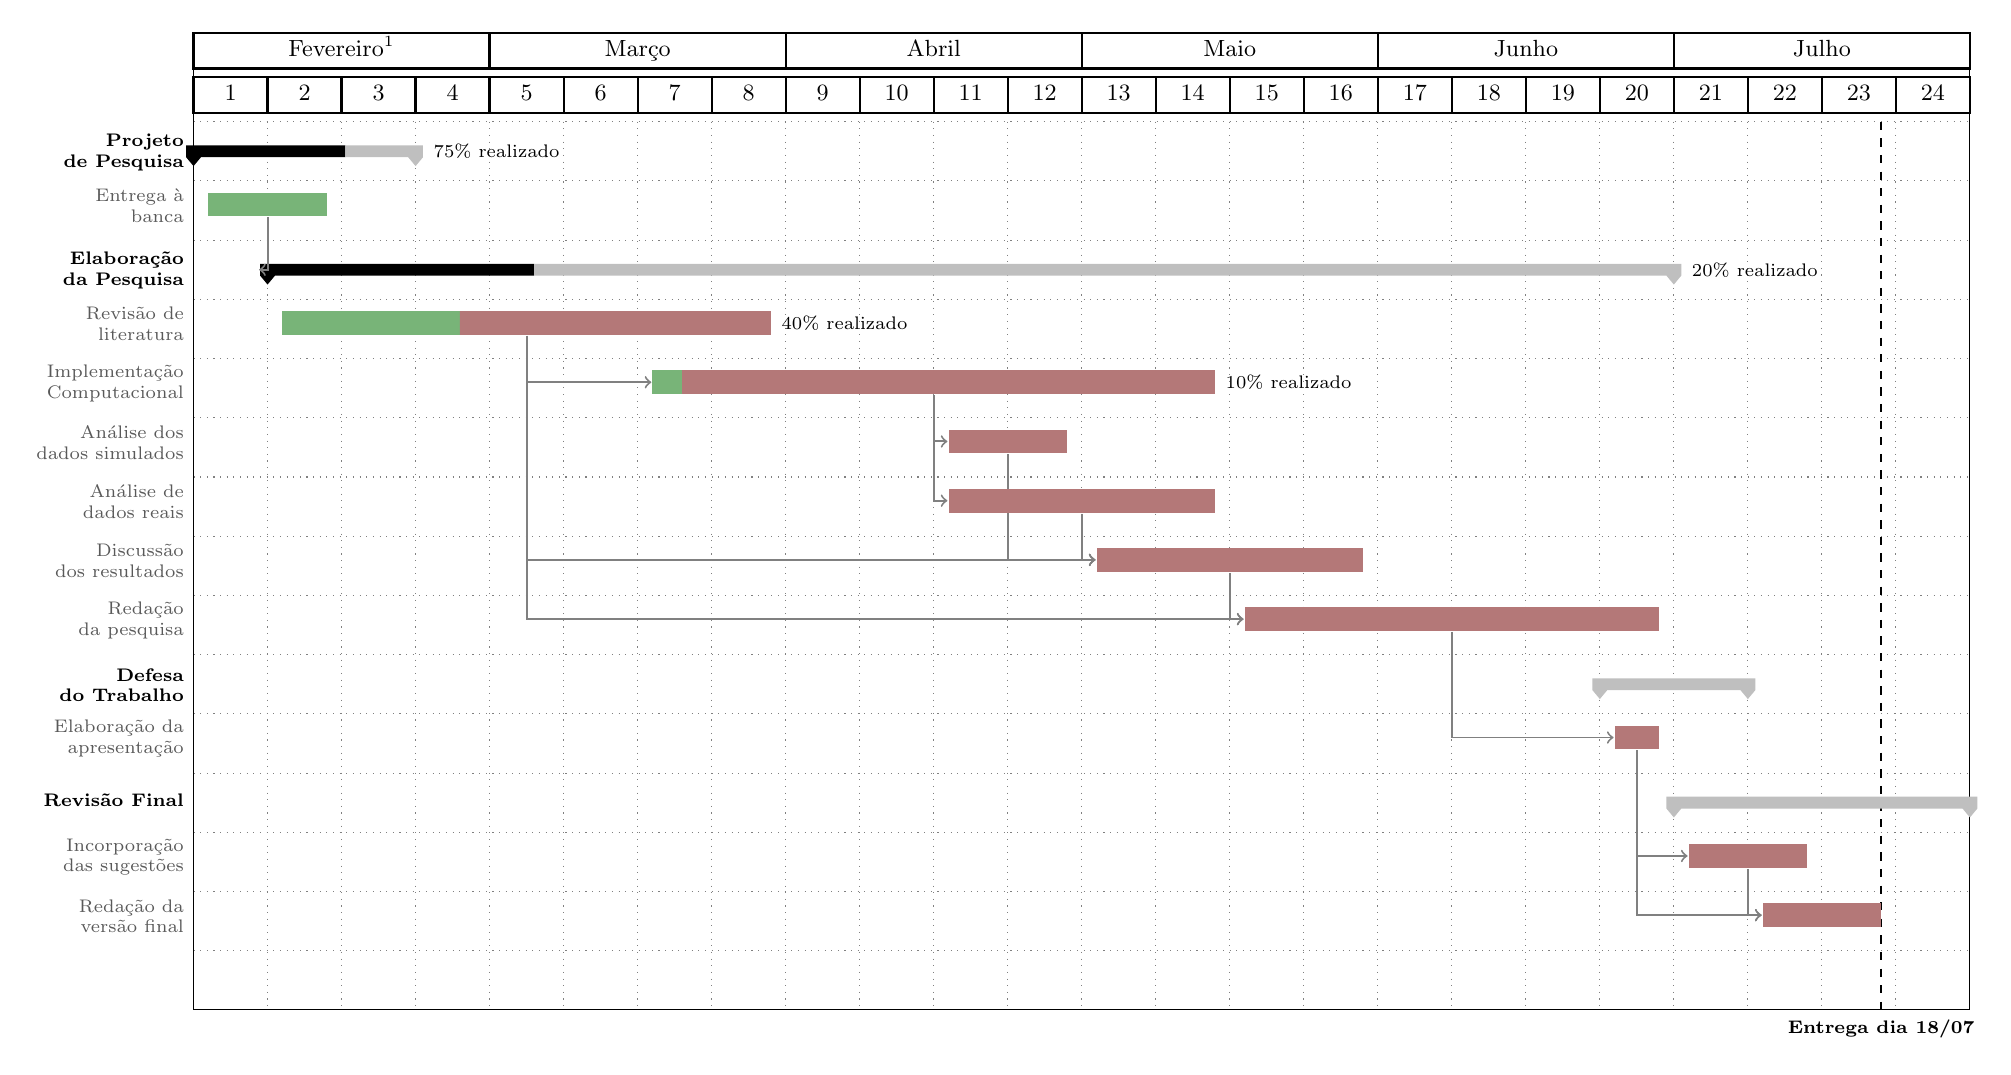
\begin{tikzpicture}[thick, scale=0.94, every node/.style={scale=0.94}]
        \begin{ganttchart}[
          canvas/.append style={fill=none},
          y unit title=0.6cm, % Size da indicação do tempo
          y unit chart=0.8cm, % Size do altura das colunas
          x unit= 10mm, % largura das celulas
          vgrid={*1{black!50, dotted}}, % grid cinza vertical
          hgrid={*1{black!50, dotted}}, % grid cinza horizontal
          title height=0.8, % Size dos dias
          bar/.style={fill=done},
          bar incomplete/.append style={fill=do}, 
          bar label node/.append style={align=right},
          bar label font=\scriptsize\color{black!65},
          group label font=\bfseries\scriptsize\color{black},
          group left peak width=0.2,
          group right peak width=0.2,
          group left peak height=0.15,
          group right peak height=0.15,
          bar height=0.6, % size das barras de tarefas
          bar left shift=.2, bar right shift=-.2,
          bar top shift=.2, bar height=.4,
          link/.style={-to, line width=0.7pt, black!50},
          link type=dr,
          today=23,
          today offset=0.8,
          today label=Entrega dia 18/07,
          today label font=\bfseries\scriptsize,
          today rule/.style={draw=black, thick, dashed},
          progress label text ={\pgfmathprintnumber[precision=0,
            verbatim]{#1}\% realizado}, 
          ]{1}{24} % 
          \gantttitle{Fevereiro\footnote{ss}}{4}
          \gantttitle{Março}{4} 
          \gantttitle{Abril}{4} 
          \gantttitle{Maio}{4} 
          \gantttitle{Junho}{4} 
          \gantttitle{Julho}{4} \\
          \gantttitlelist{1,...,24}{1} \\

          \ganttgroup[group label node/.append style={align=right}, 
          progress=75]{Projeto \ganttalignnewline de Pesquisa}{1}{3} \\
          \ganttbar[progress=100, progress label text=]{Entrega à
            \ganttalignnewline banca}{1}{2} \\

          \ganttgroup[group label node/.append style={align=right},
          progress=20]{Elaboração \ganttalignnewline da Pesquisa}{2}{20} \\
          \ganttbar[progress=40]{Revisão de \ganttalignnewline
            literatura}{2}{8} \\
          \ganttbar[progress=10]{Implementação
            \ganttalignnewline Computacional}{7}{14} \\
          \ganttbar[progress=0, progress label text= ]{Análise dos
            \ganttalignnewline dados simulados}{11}{12} \\
          \ganttbar[progress=0, progress label text= ]{Análise de
            \ganttalignnewline dados reais}{11}{14} \\
          \ganttbar[progress=0, progress label text= ]{Discussão
            \ganttalignnewline dos resultados}{13}{16} \\
          \ganttbar[progress=0, progress label text= ]{Redação
            \ganttalignnewline da pesquisa}{15}{20} \\

          \ganttgroup[group label node/.append style={align=right},
          progress=0, progress label text=]{Defesa \ganttalignnewline do
            Trabalho}{20}{21} \\  
          \ganttbar[progress=0, progress label text= ]{Elaboração da
            \ganttalignnewline apresentação}{20}{20} \\

          \ganttgroup[group label node/.append style={align=right},
          progress=0, progress label text=]{Revisão Final}{21}{24} \\ 
          \ganttbar[progress=0, progress label text= ]{Incorporação
            \ganttalignnewline das sugestões}{21}{22} \\
          \ganttbar[progress=0, progress label text= ]{Redação da 
            \ganttalignnewline versão final}{22}{23} \\
          \ganttlink{elem1}{elem2}
          \ganttlink{elem3}{elem4}
          \ganttlink{elem4}{elem5}
          \ganttlink{elem4}{elem6}
          \begin{scope}[on background layer]
            \ganttlink{elem5}{elem7}
          \end{scope}
          \ganttlink{elem6}{elem7}
          \ganttlink{elem3}{elem7}
          \ganttlink{elem3}{elem8}
          \ganttlink{elem7}{elem8}
          \ganttlink{elem8}{elem10}
          \ganttlink{elem10}{elem12}
          \ganttlink{elem10}{elem13}
          \ganttlink{elem12}{elem13}
        \end{ganttchart}
      \end{tikzpicture}
    \end{SingleSpacing}
  \end{center}

\end{landscape}

% ---
\phantompart

% ---
% Conclusão
% ---

% ----------------------------------------------------------
% ELEMENTOS PÓS-TEXTUAIS
% ----------------------------------------------------------
\postextual

% ----------------------------------------------------------
% Referências bibliográficas
% ----------------------------------------------------------
\bibliography{compois}

\end{document}
